 
\documentclass[a4paper, 12pt]{article}

\usepackage[french]{babel} 
\usepackage[utf8]{inputenc}
\usepackage[T1]{fontenc} 
\usepackage{amsmath}
\usepackage[toc,page]{appendix}
\usepackage{amssymb}
\usepackage{listings}  
\usepackage{graphicx}
\usepackage[margin=2.5cm]{geometry}
\usepackage{amsmath,amsfonts,amssymb}
\usepackage{hyperref}
\usepackage{placeins}
\lstset{
language=Java,
breaklines=true
}



\newcommand*{\plogo}{\fbox{$\mathcal{PL}$}} % Generic publisher logo

%----------------------------------------------------------------------------------------
%	TITLE PAGE
%----------------------------------------------------------------------------------------

\newcommand*{\titleGM}{\begingroup % Create the command for including the title page in the document
\hbox{ % Horizontal box
\hspace*{0.2\textwidth} % Whitespace to the left of the title page
\rule{2pt}{\textheight} % Vertical line
\hspace*{0.05\textwidth} % Whitespace between the vertical line and title page text
\parbox[b]{0.75\textwidth}{ % Paragraph box which restricts text to less than the width of the page

{\noindent\Huge\bfseries Software Project\\ Engineering }\\[2\baselineskip] % Title
{\Large \textit{Final Report}}\\[4\baselineskip] % Tagline or further description
{\Large \textbf{Project leader} : Hélène Verhaeghe}
\\
{\Large \textsc{\textbf{Group E}}\\\textsc{Aurian De Potter(Group leader)},\\ \textsc{Eddy Ndizera},\\ \textsc{Ivan Ahad},\\ \textsc{Arnaud Dethise},\\ \textsc{Ludovic Fastré},\\ \textsc{Anthony Dechamps},\\ \textsc{Geoffroy Husson},\\ \textsc{Jonathan Legat}} % Author name

\vspace{0.5\textheight} % Whitespace between the title block and the publisher
{\noindent \Large \textbf{INGI2255}}\\[\baselineskip] % Publisher and logo
}\\

}
\endgroup}


\clearpage
\setcounter{page}{0}
\begin{document}


\titleGM
\tableofcontents
\newpage

\begin{figure}[h]

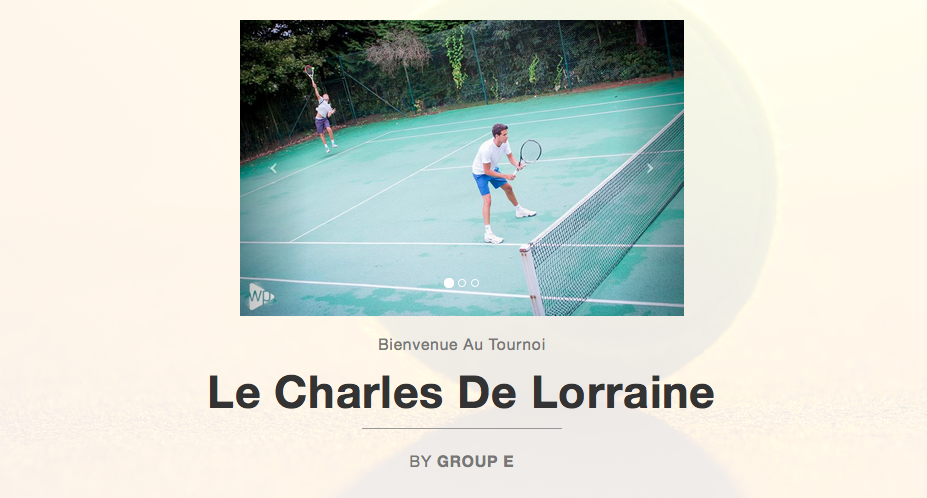
\includegraphics[scale=0.4]{accueil.png}
\end{figure}
\section{Introduction \& Presentation of The Project}

Each year, the ASMAE non-profit organization organizes a tennis tournament that gathers many players during one week-end. Last September, representatives of this organization queried our help to revamp their website. This website is used for the tennis players to register themselves for several kinds of tournaments. However, their current website was old and started to show its limits.\\

Thus, our goal is to create a new revamped website that allows players to register, court owners to lend their own courts for the sake of the tournament, and having a better experience of the utilization of the website, as it will need to be easy and trivial to use. One important update is to have a fully working staff part to manage the tournaments, the players, the courts, etc. \\

This report will describe everything you need to know about the software in general and all the important information of how it works and how it has been built. \\

We will first start by listing all the optional and mandatory  requirements that we were asked to implement and which of those have indeed been implemented. We will also add further explanation about our implementation choices for some of the requirements. \\

Then we will dedicate the third section to scan through all the processes of development of the project. This section will be divided in four parts. The first subsection will be the global organization of the project and the tools that we chose to use to build the software. In the second subsection, we will present you the website in general, where we will show you everything you need to know about it, and all the important functionalities that it required to have. The third one will be a more technical part that is the programming architecture, and finally we will explain how we scheduled all the tasks that were necessary for the development of the project.\\

\newpage
\section{List of All The Requirements}
We will now list all the elements that we were asked to implement in our software. The requirements had different priorities, divided into \textit{Must Have, Should Have, Could Have and Would Like to Have}. \\

However, rather than dividing them in those four categories, we decided to divide them into mandatory requirements and optional ones (the optional ones are in italic). \\

We also sorted  them depending on if they're functionnal or non-functional. Note that we added some requirements not explicitly said by the clients but that we consider to be relevant for the project (such the privacy parts).The \textit{non-functional} requirements answer to the question "how should it be done" while the \textit{functional} ones represent actual functionalities.\\

Notice that all the \textit{Must Have} requirements have been implemented. For the \textit{Would Like to Have} requirements, we thought they required too much time and we decided to focus on the top priority requirements. Among the \textit{Should Have} requirements, the automatic generation of knock-off has been implmemented. QUID DES COULD HAVE ET SHOULD HAVE?\\
\subsection*{Functional}

\subsubsection*{User}
	
	These requirements describe functionalities for a player that wants to take part in one of the tournaments. Among them, a user must be able to enter his information in a form containing all the important fields, to register for a tournament, to register one of his courts if he is an owner, etc.\\
	
	\begin{itemize}
		\item The user can enter his data (including special characters) - yes
		\item The users can register to a tournament as a pair, selecting his category - yes
		\item \textit{The user can reuse old data linked to his email address to automatically fill a registration form} - yes
		\item The user can register for activities during a tournament (barbecue, etc) and choose preferences such as taking responsibilities and payment method - yes
		\item \textit{The user can register on a tournament alone and be matched with another player} - yes
		\item The user can register a personal court as being available for the tournament - yes
		\item \textit{Users who registered their own court can see information about players who will play on those.} - yes
		\item \textit{The user can use a payment method among several options} - yes
		\item The user can leave a comment when registering - yes
	\end{itemize}

\subsubsection*{Administrator}
    Here, we have the requirements that concern all the abilities that an administrator account must have. More generally, an administrator must be able to control most of the website, that is the registrations, the other admin accounts, staff accounts, etc. An administrator must also have the ability to manage tournaments in general. An administrator account has more rights than staff accounts, as they must manage almost every aspect of the website.\\ 
    
    \begin{itemize}
    	\item An admin can start or close a tournament - yes
    	\item An admin can close the registration for a tournament (and trigger the creation of pools) - yes
    	\item An admin can create an admin account - yes
		\item An admin can create a staff account - yes
		\item An admin can delete an account - yes

    \end{itemize}
    
\subsubsection*{Staff} 
    A staff account is used by the members of the ASMAE organisation. They make sure the tournaments are going as expected, they send important information to the players for their matches, they can assign courts to players, etc. For example, we made it possible for staff members to  broadcast a message to all participants so that they can send new information and reminders about the tournaments.\\\\
    
    \begin{itemize}
    	\item After a pool has been generated, a staff member can manually reorganize it - yes
		\item A staff member can manually assign a court for each match, or modify it in case of raining - yes
		\item A staff member can use a mail list / newsletter functionality - yes
		\item A staff member can enter or edit match result data - yes
		\item A staff member can see all the user informations (except credentials) - yes
		\item A staff member can visualize and print the evolution of the tournament in a fashionable and displayable form (both graphic and text), step by step using the knockoff, and print the pool matchup sheet - yes
		\item A staff member can access the courts list - yes
		\item \textit{A staff member can manually match two users as a pair for a tournament}
		\item \textit{Common page for staff members} - yes
		\item \textit{Files sharing between staff members} - yes
		\item \textit{Communication channel between staff members}
    \end{itemize}
    
\subsubsection*{System}   
     This represents the functionalities of the website.
    \begin{itemize}
    	\item \textit{The system can create pools and match ups} - yes
		\item \textit{The system must confirm email addresses} - yes
		\item \textit{The system must query AFT rankings}
		\item \textit{The system can create smaller pools when it rains}
    \end{itemize}
    
\subsection*{Non-Functional}
In this subsection are listed the requirements that are more technical. Those are necessary so that the website works correctly. 

\subsubsection*{Interface}
	
	\begin{itemize}
		\item The interface must be user friendly - yes
		\item \textit{The interface must be mobile friendly} - yes but some input boxes are not
	\end{itemize}

\subsubsection*{Documentation}
	
	\begin{itemize}
		\item The software must be well documented - yes
	\end{itemize}
	
\subsubsection*{Privacy}
    
    \begin{itemize}
    	\item Turn off indexation of private data - yes
    \end{itemize}



\subsubsection*{Reasons to use a new software}


	\begin{itemize}
		\item Interface is easier to use - yes
		\item Many tasks are automated - yes
		\item Code base is simpler and more modular if future modifications are wanted - yes
		\item More flexibility for users such as solo enrollment - yes
	\end{itemize}


\newpage


In this section, we will present to you our website and all the important aspects of it, such as how we developed it, how it looks like, what kind of features it contains, etc.

\subsection{Organisation and Tools used}

We are briefly going to explain the way the group decided to develop the project. After being introduced to the project by our customers, we had to choose between a few development methods to use throughout the making of the software. The group decided pick the \textbf{Agile} method. \\

The first step of this method is writing down user stories. These are used to represent all the functionalities of the software which is the website. Afterwards, the group has to discuss about the importance and the difficulty of each user story, and then decide which of them have the top priority. \\

When this is done, we will use a kanban to organize the process of the project. The kanban contains all the user stories, and is divided into the following categories : “To do, doing this iteration, done this iteration, and done”. Every member of the group picks the user stories he thinks he is able to implement, so it allows us to know which member has done each task. For the kanban we will use the \textbf{Trello} Website (www.trello.com). \\

The programming language we decided to used was Python, with the \textbf{Django} framework.\\

We would use the third version of Python, and the 1.8 version of Django. Lastly, we would also use the \textbf{Bootstrap} framework for the design of the website (the css part essentially). \\

To easily share the project’s code, we will use a Control Version System, which is in this case \textbf{Git}. Git, and its underlying service called GitHub(www.github.com), is preferred since it allows us to make private repositories. 

We also decided to divide the project into 4 iterations, corresponding to the 4 phases presented to us. With the Agile method, there will be a working deliverable for each of these phases. Through each iteration, we will have to add up functionalities to the working project, until each of them is implemented.  \\

To host a live version of the website, we used Heroku (www.heroku.com).\\

There are a few reasons why we picked this way of working. First of all, this method was genuinely our first choice since it is the one we are the most comfortable with, as we have been using such a method for a few projects now. Moreover, we liked its versatility since every member of the group has to be involved in every aspect of the project. Furthermore, after each iteration, we will have a meeting with our Assistant. This meeting will allow us to get a feedback of each deliverable. The feedback received will then help us to know if changes need to be done, if there are unnecessary things, or if our project is moving towards the right direction. Finally, with the Agile method, we will first implement all the “must have” functionalities, which allow us to focus on the core of the software, and then add up the functionalities with less priority. \\

\begin{figure}[h]


\includegraphics[scale=0.5]{onglets.png}
\end{figure}
\section{Development and Implementation}
\subsection{The Website, Its Functionalities}

In this section, we will show you the fully built website and we will explain everything you need to know about its functionalities. We will seperately explain the functionalities with the help of screenshots and sequence diagrams. To get a look at the live version of our website, you can click here : http://sep2015e.herokuapp.com. \\



\subsection*{Registration of a player}

\begin{figure}[h]
\caption{\label{register} Registration form}
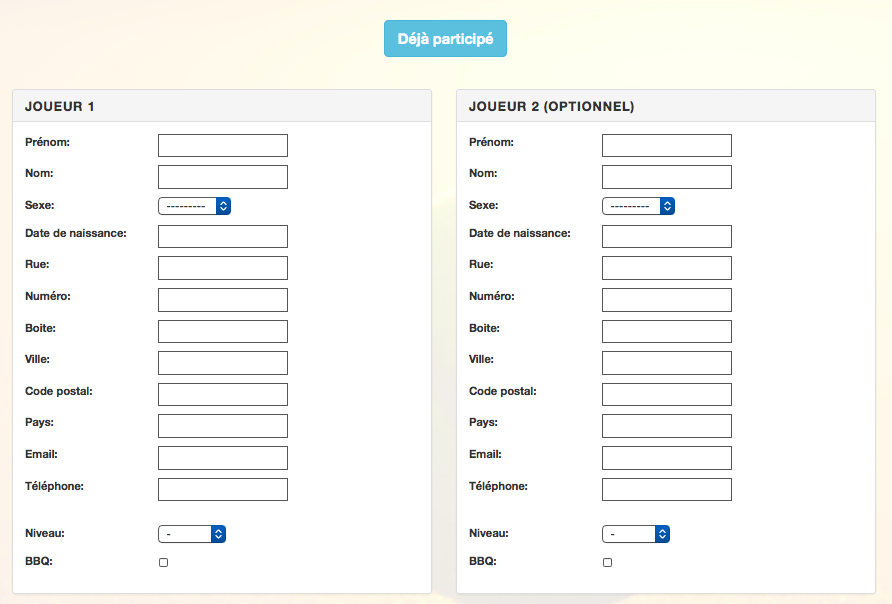
\includegraphics[scale=0.5]{playerform.png}
\end{figure}
\FloatBarrier

The first main and most important functionality of the website is the registration of a player, as the users will usually visit the website to to do and to assign themselves to a tournament.\\

\begin{figure}[h]
\caption{\label{obligatoire} Required fields}

\includegraphics[scale=0.7]{obligatoire.png}
\end{figure}
\FloatBarrier

To do so, a user must fill in the form with all the required fields. Once this is done, the system will check if all the mandatory fields have been filled. If not, some warning will appear to precise which field must be correctly filled, as you can see in the screenshot above(Figure \ref{obligatoire}). Once all the fields are correct, the user is redirected to a page that shows a summary of all the payments for him, allowing him to check what he is going to pay afterwards.. It is important to note that we have implemented a smart registration, where a player is automatically assigned to a tournament according to his information. In figure \ref{recap}, you can see an example of how the information is presented after validation. Also note that the payment choice is chosen after a user has entered and validated all his information.\\

If a member is registered alone for a tournament, a staff member can eventually match him with another member that is alone.\\

The user can also re-use old data linked to his email address to automatically fill a registration form. To implement this, we added a link on the registration forms so that previous participants can use their old information for new ones. All they have to do is give  their previously used address. Another use of the email address of a user is when a participant submits his registration form, the software sends an automatic email to confirm that the player has a valid email address.\\

To make it possible for a user to look for other users or to check the list of all the available courts, we added a functionality that allows to look for players and courts, but also pairs. We then added a list of all the players and all the courts.(SCREEN)\\

We have built a sequence diagram, at figure \ref{playerseq}, that illustrates how the registration of a player goes.\\
\begin{figure}[h]
  \caption{\label{recap} Summary of player information}
  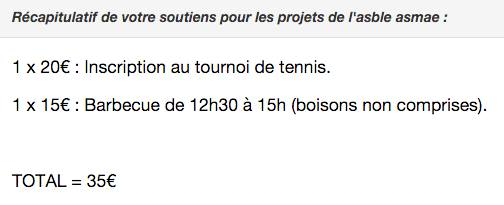
\includegraphics[scale=0.7]{recap.png}
\end{figure}

\begin{figure}

   \caption{\label{playerseq} Sequence diagram}
  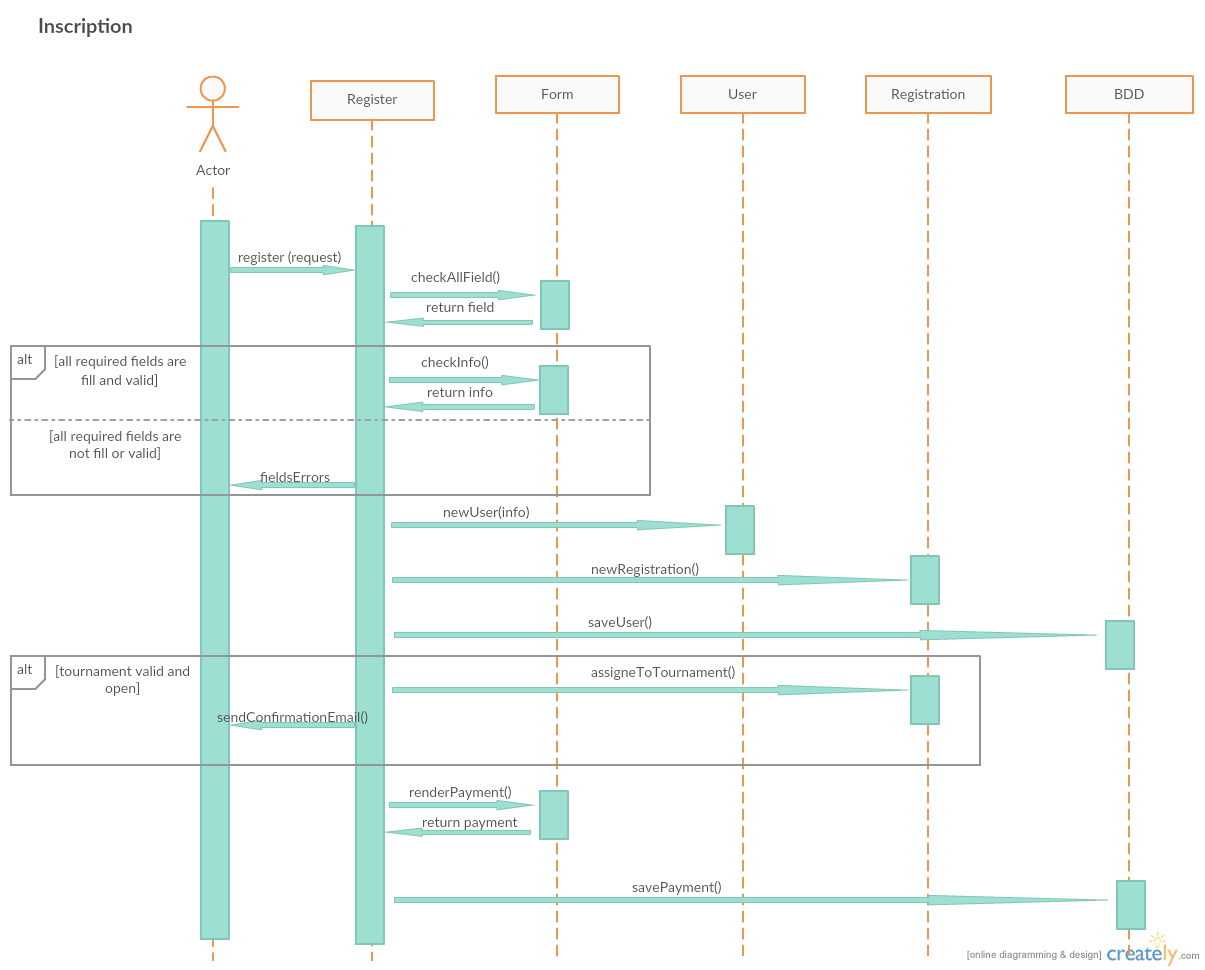
\includegraphics[scale=0.4]{Inscription.png}
\end{figure}
\FloatBarrier
\newpage

\subsection*{Owner Court Registration}

One other main reason why users usually visit the website is to register their own court to make them available for the different tournaments of the week-end event. We will see how one can register a court.\\


\begin{figure}[h]
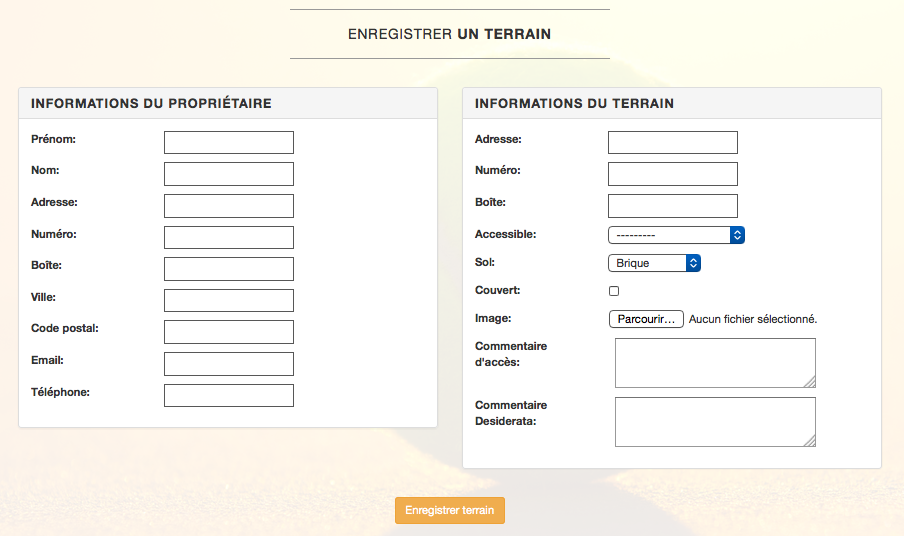
\includegraphics[scale=0.5]{registercourt.png}
\end{figure}

When clicking on the "\textit{Terrains}" tab of our website, a user gets to a page as presented above. A form is available to be filled with the information of the owner of a court that must be registered. Once this is done, there is a second form to be filled with all the information of the court to be registered, such as its address, the surface of the court, a picture, etc.\\

\begin{figure}[h]

\includegraphics[scale=0.5]{courtmail.png}
\end{figure}

This message above is shown when the registration is completed, an confirmation email is then sent to the owner.\\

We have built a sequence diagram, at figure \ref{courtseq}, that illustrates how the registration of a court is done in a more technical way.\\

\begin{figure}[h]
   \caption{\label{courtseq} Sequence diagram for a Court registration}
  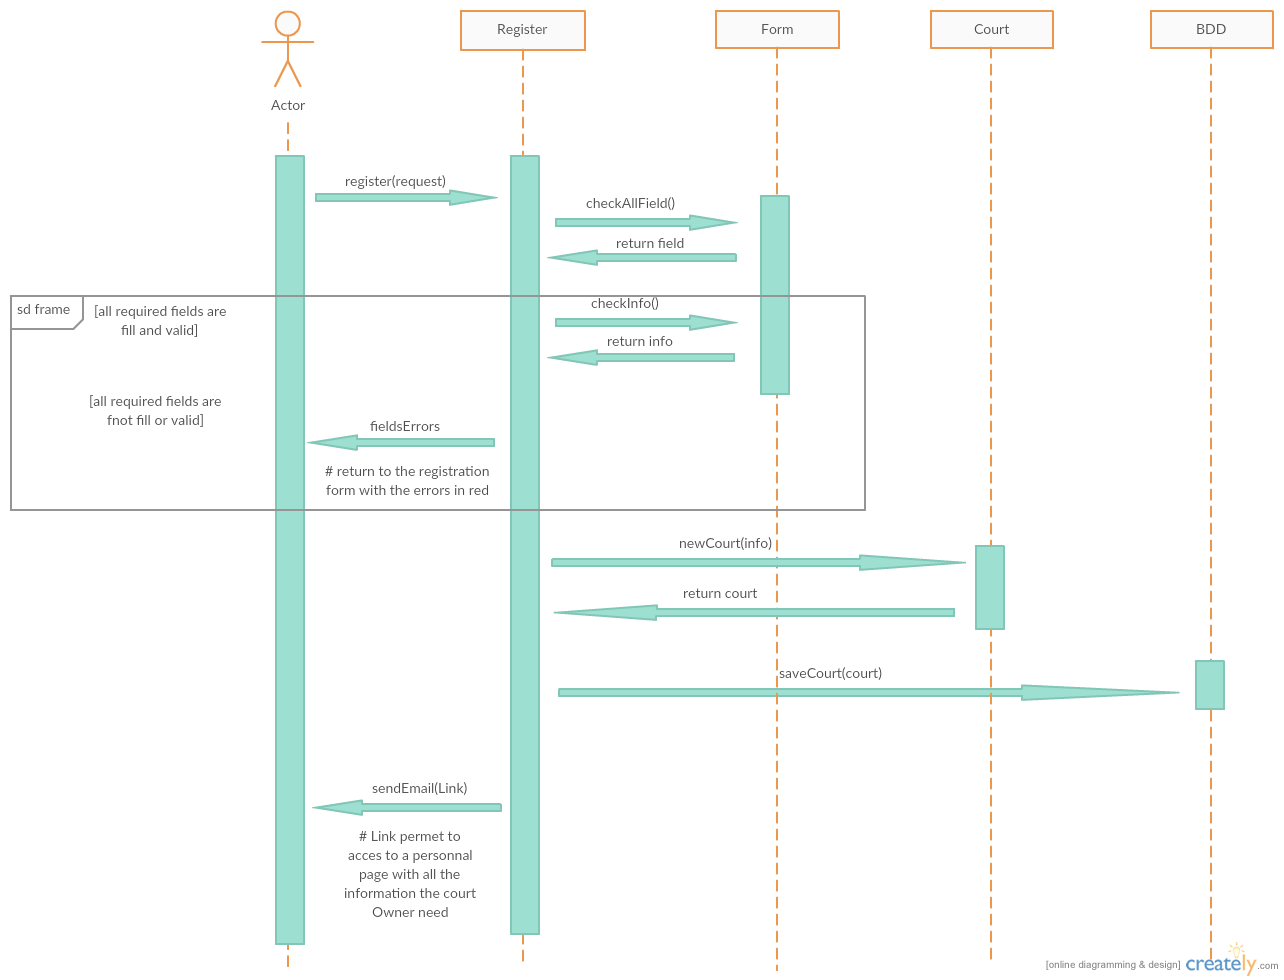
\includegraphics[scale=0.4]{courtseq.png}
\end{figure}

\FloatBarrier
\newpage

\subsection*{Staff Role}

\begin{figure}[h]

\includegraphics[scale=0.5]{staffaccueil.png}
\end{figure}
\FloatBarrier
A staff has a key role for the management of the website. We made sure that his abilities were as wide as possible. The staff part of the website is recognizable thanks to its different and darker background. Let us see what a staff user can manage in the website.\\

\subsubsection*{Editing a Player's Information}
\begin{figure}[h]

\includegraphics[scale=0.5]{listeplayers.png}
\end{figure}

A staff member can check and edit the list of all the registered players by clicking on the "Joueurs" tab. There are three lists in this page, a regular list of all the players, a list of the pairs that aren't assigned to a tournament yet, and players that are alone. When clicking on the name of a player, one gets access to a form with all the fields that are editable, as well as deleting a member if necessary.\\

\subsubsection*{Checking the Courts' information}
\begin{figure}[h]
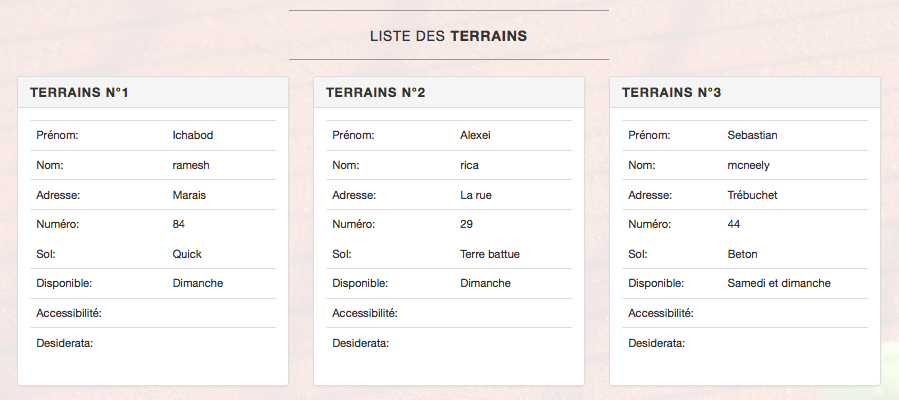
\includegraphics[scale=0.5]{courts.png}
\end{figure}
A staff member also has acces the all the courts' information available at the "Terrains" tab that were registered for the week-end, as you can see in the screenshot above. 
\subsubsection*{File Sharing and Communication between staff members}

In this section, we will describe a functionality that allows a good communication between the staff members, as requested. The website contains a page reached by clicking on the "Accueil tab" in which we implemented a functionality that allows to exchange messages. We also added a feature that allows to share files that they can upload/download. The staff members already have other means to communicate, so these two features should mostly be used for very important announcements. They are available on a dedicated page. You can see in figure \ref{annonce} below how a staff member can put an announcement, and how one can upload files in figure \ref{file}.\\

\begin{figure}[h]
  \caption{\label{annonce} Announcement creation}
  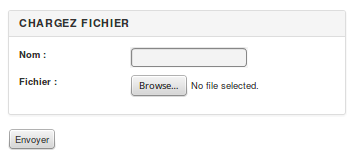
\includegraphics[scale=0.7]{annonce.png}
\end{figure}
\FloatBarrier
\begin{figure}[h]
  \caption{\label{file} File sharing}
  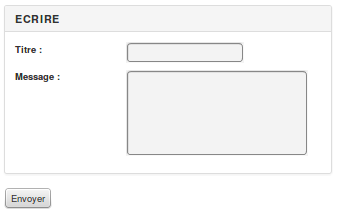
\includegraphics[scale=0.7]{fichier.png}
\end{figure}
\FloatBarrier

 \newpage


\subsubsection*{Tournaments managing}
The last key role for a staff member is everything that is related to the tournaments management. A staff member has access to the tournaments managing page by going to the "Tournois" tab.\\

\begin{figure}[h]
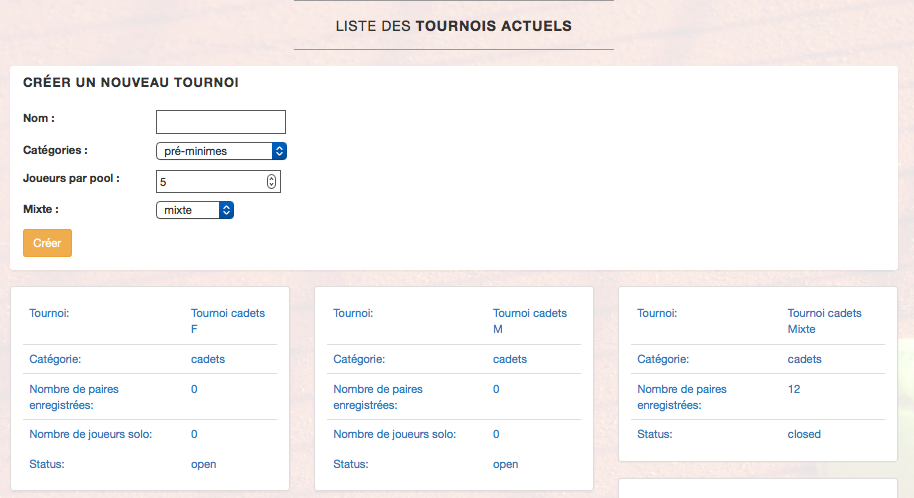
\includegraphics[scale=0.5]{stafftournament.png}
\end{figure}
\FloatBarrier
The main feature is the creation of a tournament, as presented in the screenshot above. A staff member must choose the tournament's name by filling the required field, must choose the level of its participants, the number of players per groups and finally if the tournament is mixed or not.\\

Afterwards, a list of all the created tournaments is available on the same page, with all their important information. By clicking on a tournament, one gets access to every important feature of each of them. Let us see what are those features that a staff member can use to edit/add information.\\

\begin{figure}[h]
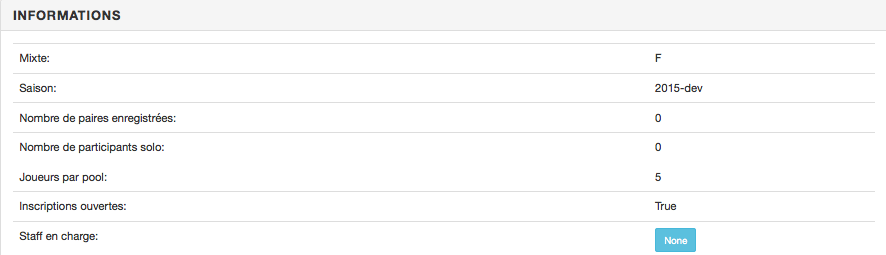
\includegraphics[scale=0.5]{infotournament.png}
\end{figure}
\FloatBarrier
First, there is a summary of all the information of the chosen tournament. There is a button that allows to assign staff members to the tournament as its managers.\\

\begin{figure}[h]
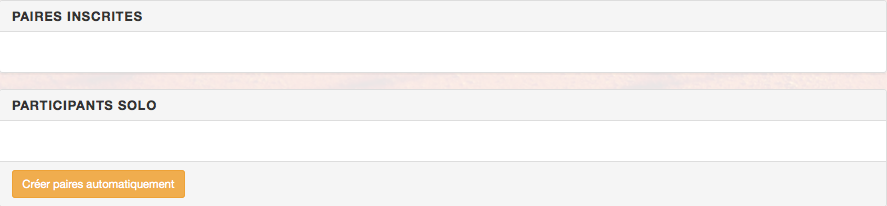
\includegraphics[scale=0.5]{participtournament.png}
\end{figure}
\FloatBarrier
There is also the list of the fully registered players by pairs, and a list of all the players that are alone. From that point, we implemented a feature that allows a staff member to automatically match single players with each others to form a pair.\\

\begin{figure}[h]
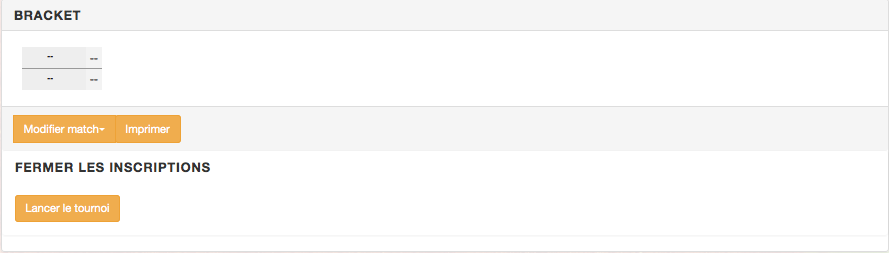
\includegraphics[scale=0.5]{bracket.png}
\end{figure}
\FloatBarrier
When all the players are registered, the tournament is set to be launched, and the groups containing all the registered players will be available. The knockoff tournament is represented in the "bracket section" that you see on the screenshot above. A staff member can visualize and print the evolution of the tournament in a fashionable and displayable form (both graphic and text), step by step, using the knockoff, and print the pool matchup sheet. When closing the registration for a tournament, a pdf is generated with all the pools. It was done this way so that the visitors can print the pdf themselves. Plus, the pdf is only generated once. The staff members can see on the website the pools and the corresponding fixtures, they can also edit the matches, as they have a global view of the pools. \\

Upon encoding all the scores of the matches in a pool, the winner of this group is displayed in green and the knock-off tournament is created in the database. Plus, it is  possible to see the bracket with a pretty graphical version. The players that are the winners of a group will then get to the bracket.\\

The sequence diagram at figure \ref{tournseq} illustrates better how the life cycle of a tournament is. More generally, it shows how players are added into groups, how the knock-off tournament is created, how the tournament is created, etc.\\

\begin{figure}[h]
   \caption{\label{tournseq} Sequence diagram for tournament}
  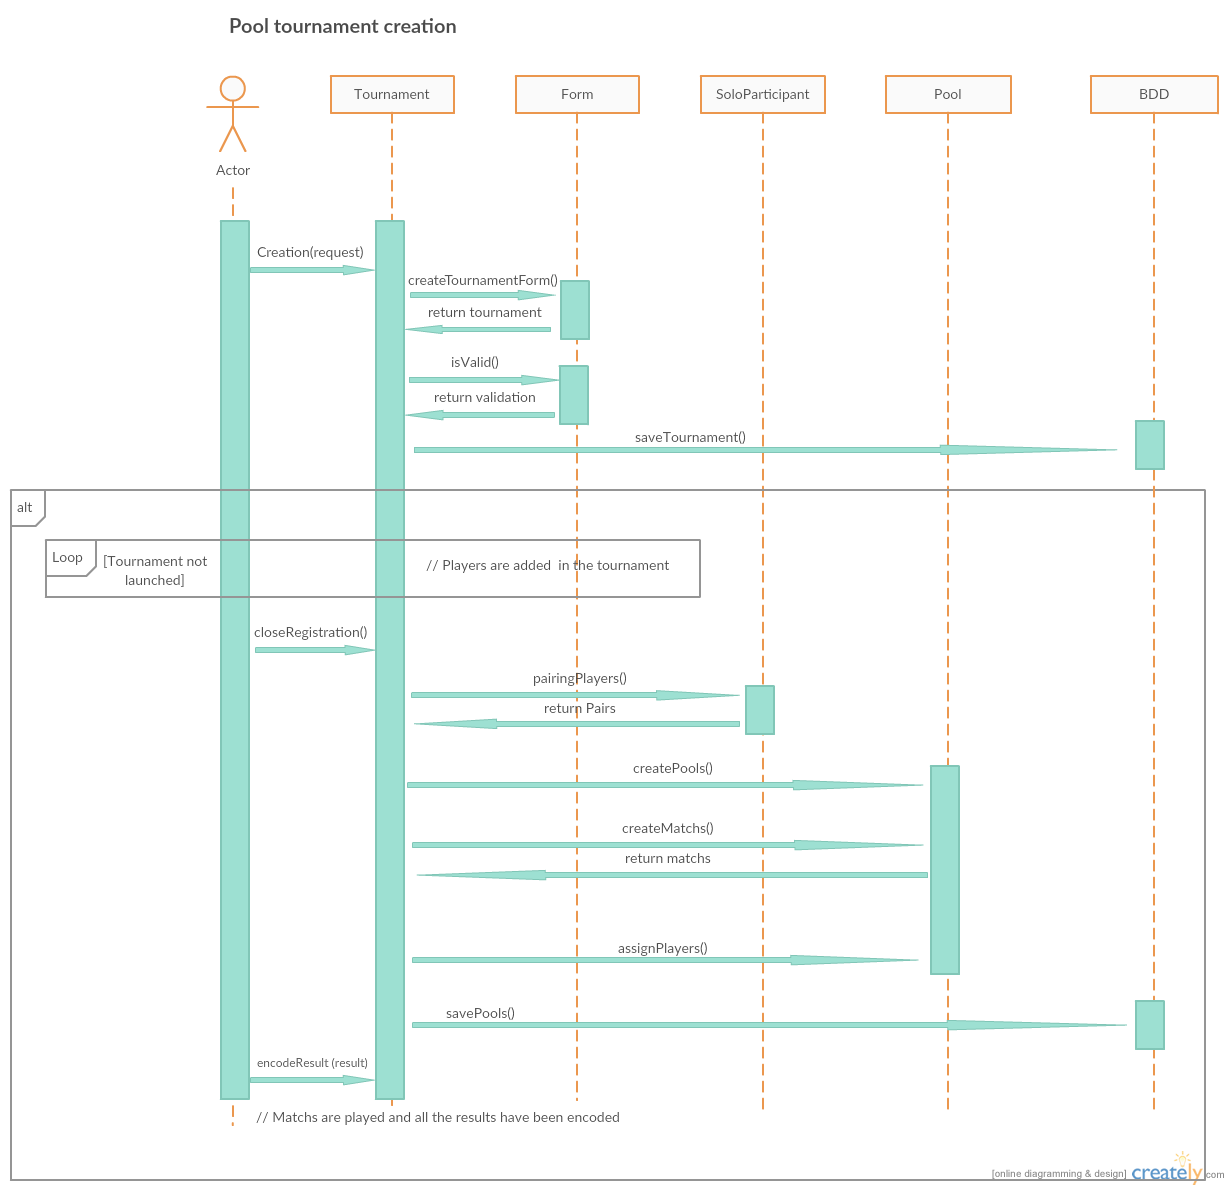
\includegraphics[scale=0.4]{Tournament.png}
\end{figure}
\FloatBarrier
\newpage


\subsection*{Administration part}

An administrator is in top of the hierarchy when it comes to abilities on the wbesite. In this case, administrators are very important, as they are able to create staff and admin accounts, to delete other staff and admin accounts, and to delete regular accounts. Plus, it can modify the credentials of all the users that are registered.\\

However, the most important role for an administrator is that it is the only type of account that is able to close a tournament.

\subsection*{For Future Developers}

In case future developers would want to modify anything on the website, we made a wiki that explains everything about the project and the code. The wiki is available here :https://github.com/ivanahad/sep2015E/wiki, however we will not discuss about it in this report, as the wiki already contains consistent information.

\subsection{The Architecture}
This section will be dedicated to explain the more technical parts of our software and its underlying programming particularities. It will be divided in two parts. The first one will give further details about how tournaments, players, users, courts, and other important objects are represented in the database, and how those objects are linked together. The second one even more technical, as it explains how the software is structured, and how our team programmed all the important parts to build the website.\\


\textbf{To get access to the code of our project}, you can click on the link to our \textit{Github} repository : https://github.com/ivanahad/sep2015E\\

\newpage
\subsubsection{The Object-Relational Mapping}
Fig.1 shows our ORM diagram. It gives an idea about how the different objects used by the website are linked together. We will give a brief description of what the object represents and its relations to others.\\

The user represents a player participating in the tournament. It is characterized by a name, an email, an address and the level of the player (meaning how good he is at tennis).\\

A pair is formed of two users. A single pair can only participate in one pool of the tournament. A pool contains pairs and their match (matchups between pairs). A match is characterized by the pairs confronting each other and the court in which they will play. The court object contains information about the court owner, the address of it and finally some comments about it like the type of surface.\\

As we said, a tournament is composed of pools but also of a knock-off tournament that we called tree in our diagram. Moreover, a tournament is defined by its category. Finally, the tree is composed of nodes that is basically a pair of two users.\\

A staff, similarly to a user is characterized by it's name, address, contact (phone and email) but also by it's password. Also a staff is part of group representing the actions he can do. \\

A message is defined by it's author which is a staff member, by it's title and by it's content (text). A file is defined by it's title, it's owner and the file.\\

This concludes the description of our ORM diagram. 

\begin{figure}[ht!]
\caption{\label{orm2} Revamped ORM Diagram}
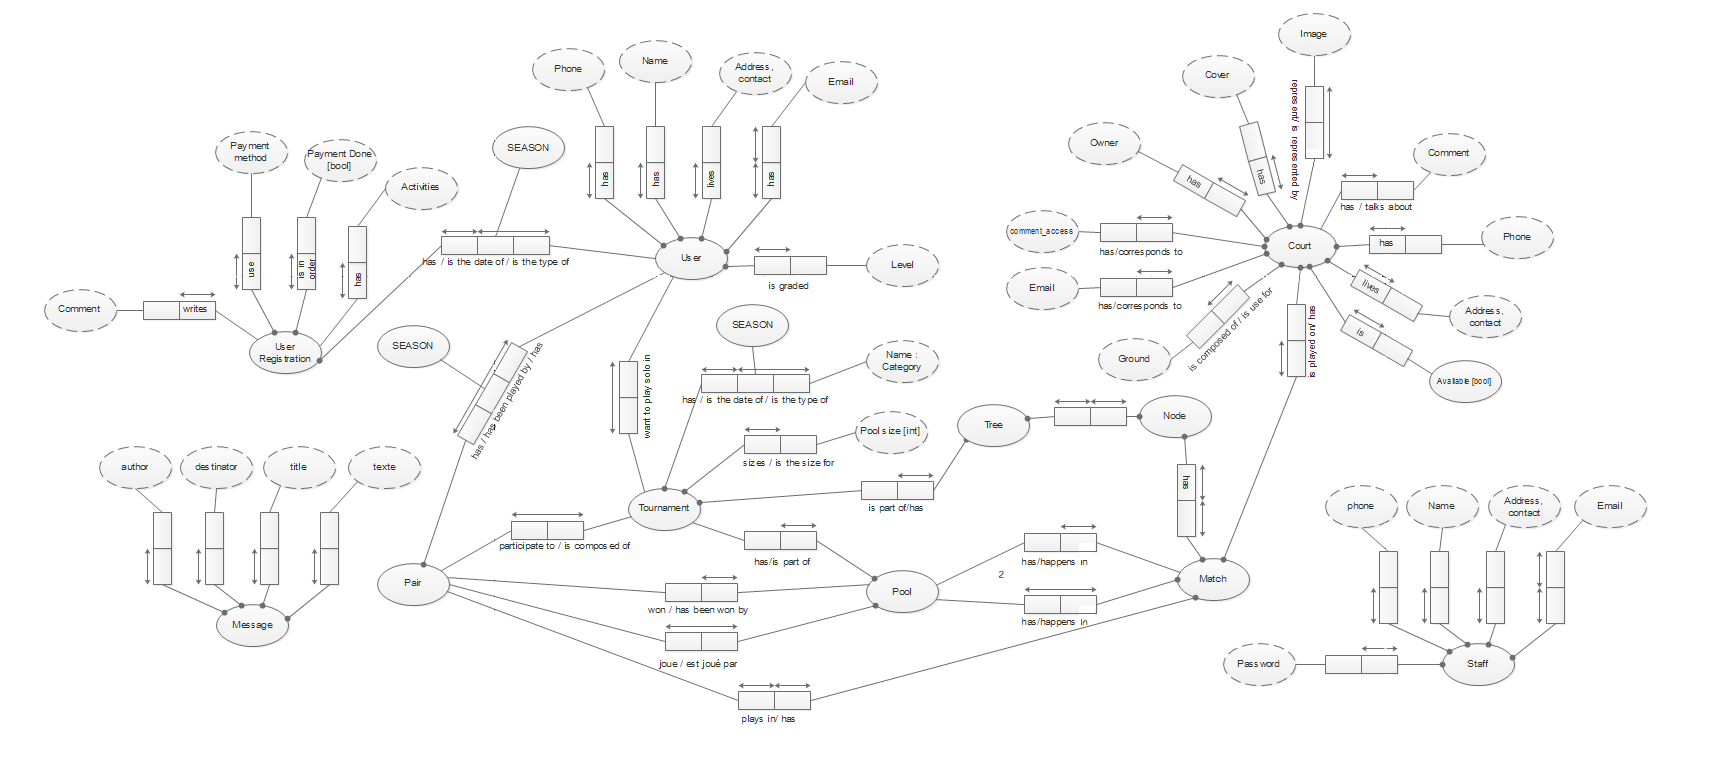
\includegraphics[scale=0.60, angle=90]{ormp2.PNG}
\end{figure}
\FloatBarrier


\subsubsection{The Uniform Modeling Language}
UML
\begin{figure}[h]
	\centering
 	\caption{\label{uml} UML diagram}
	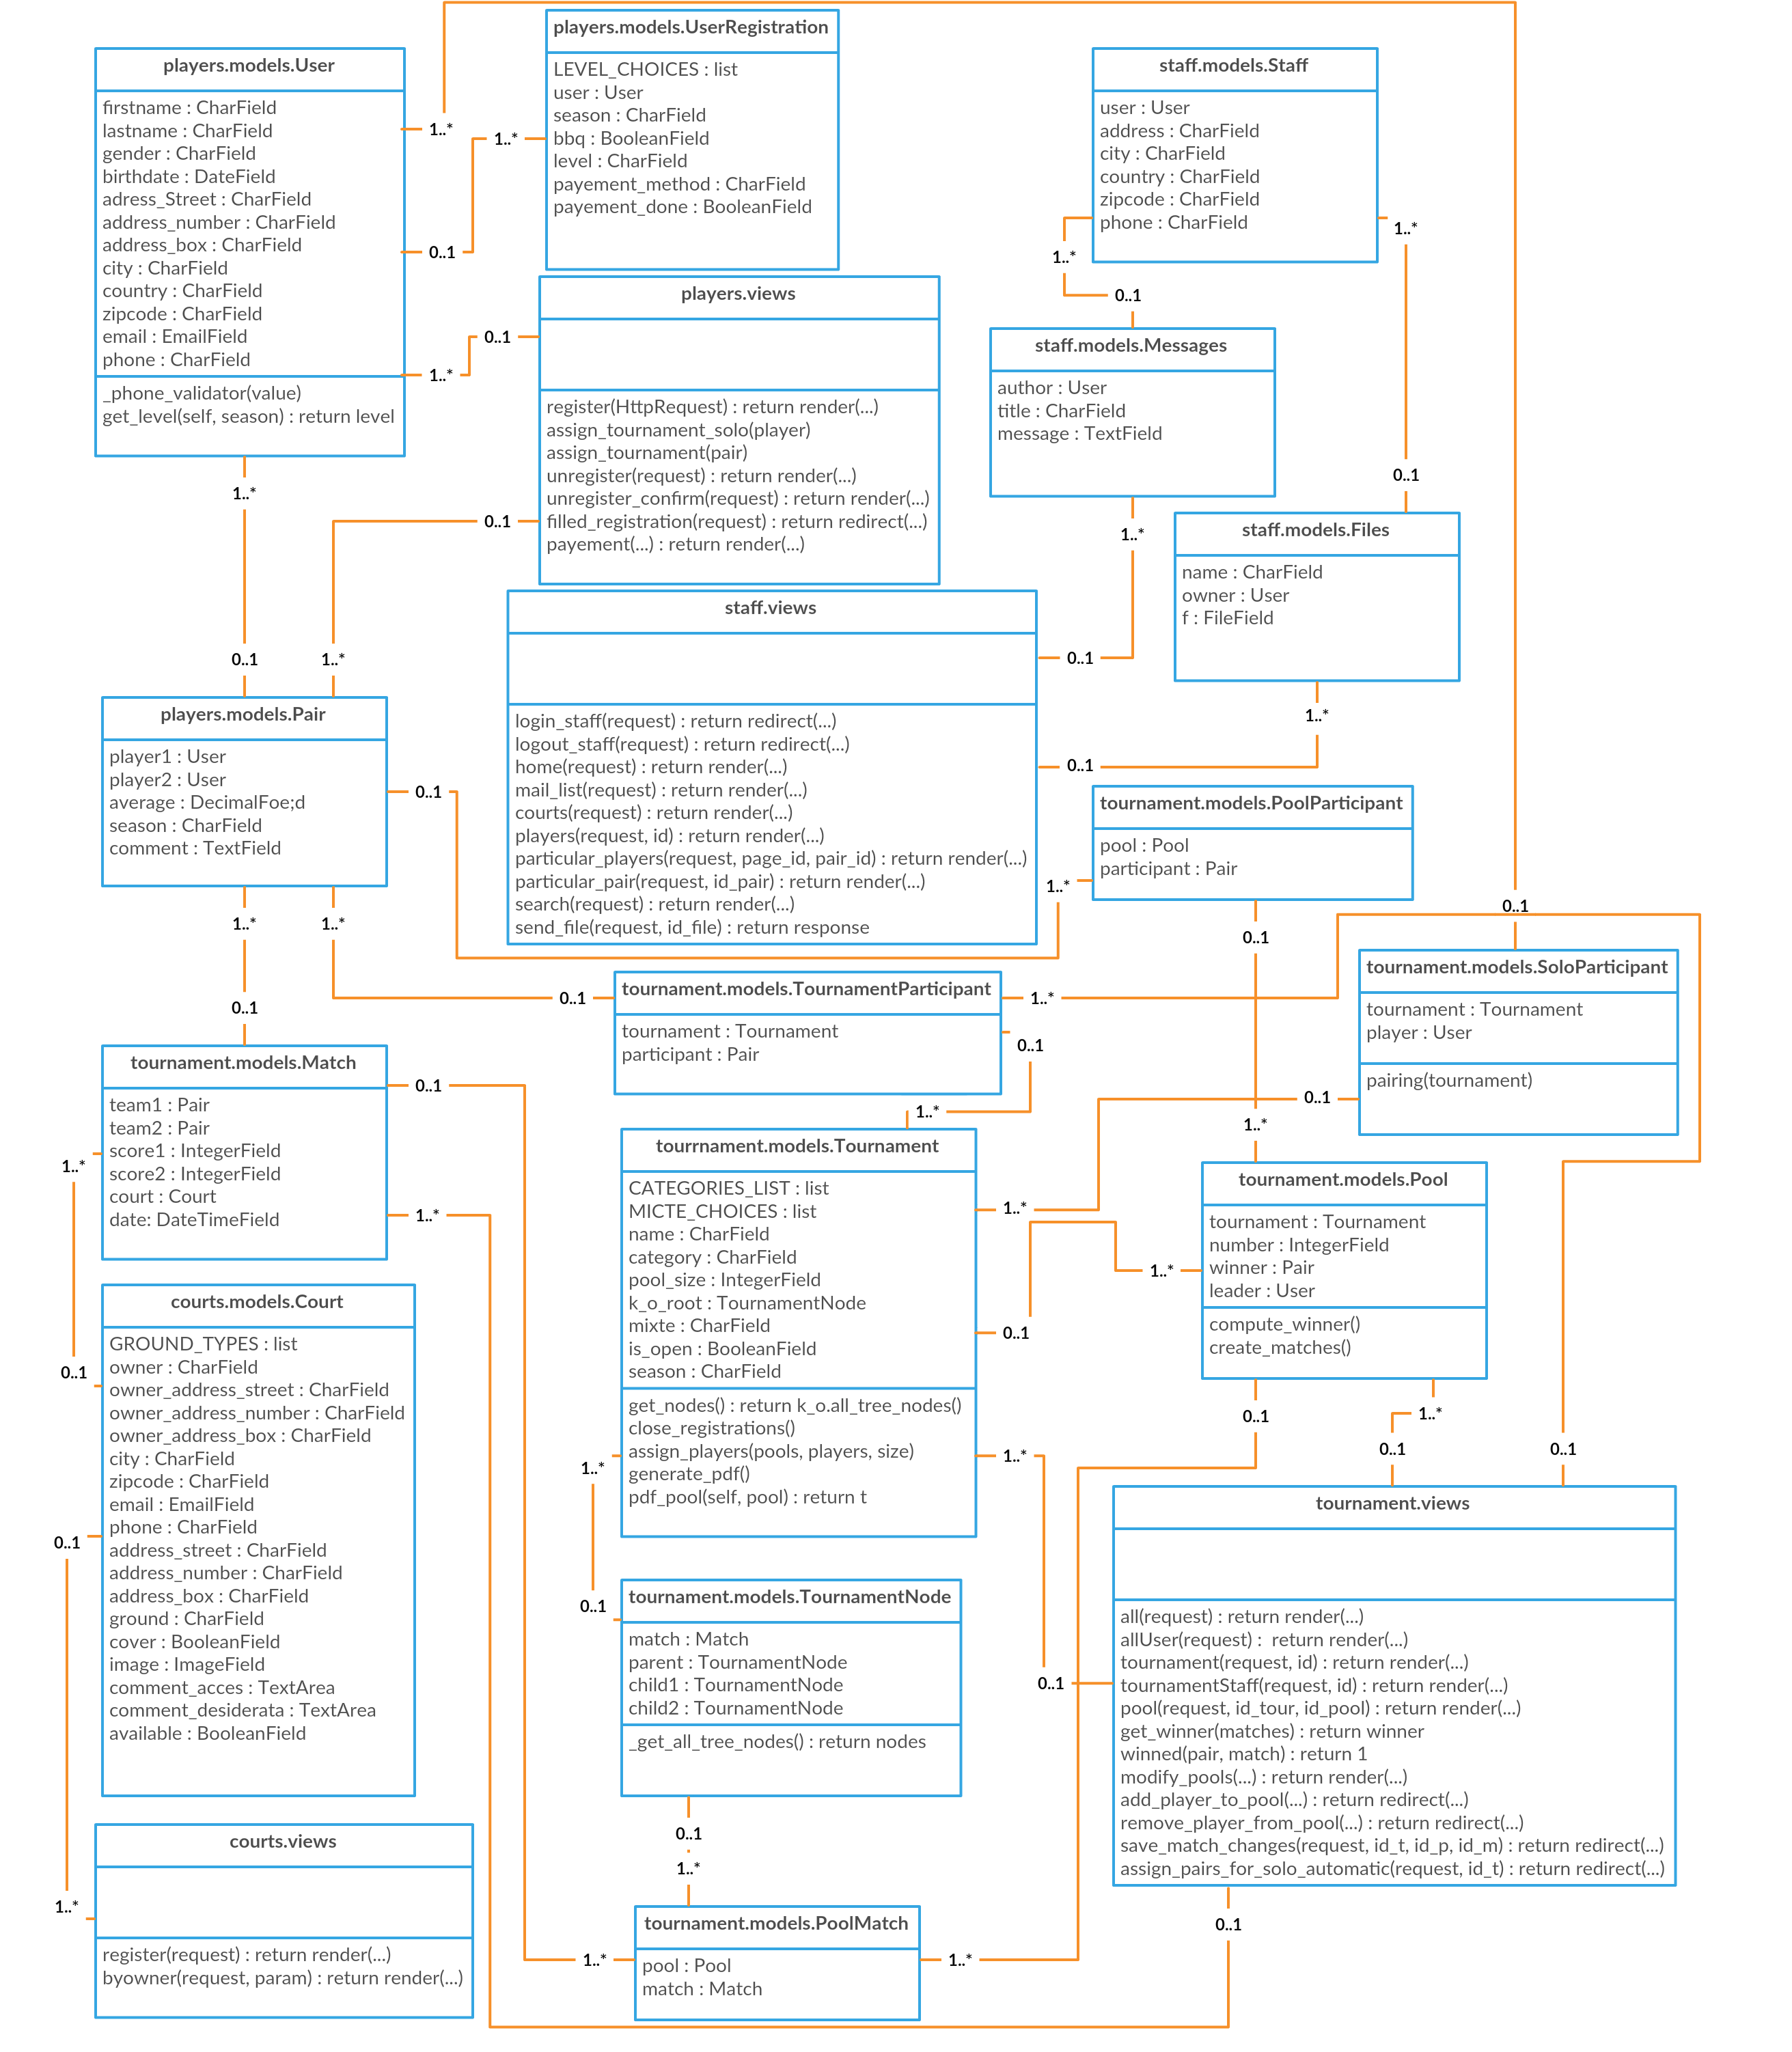
\includegraphics[scale=0.2]{Class.png}
\end{figure}
\FloatBarrier

\subsection{Evolution of the Project}

In this section, we will briefly describe the progress of the website through four phases.\\

First off, we gathered to speak about the project in general. During the first meeting, we had to decide which tools we were going to use and how we were going to program our website (mainly the programming languages to be used). The summary of what we decided is in section 3.1.\\

After deciding all the key elements for the project, we started programming the software. We implemented what we considered to be the base of the project so that we have something to start with. This consisted of the creation of the different pages needed to register a player, a court and the staff and admin pages. The database was also created with the different tables for the user, the staff, etc. We chose a template design that was subject to change all along the project.\\

For the rest of the development, our task was to fix all the bugs and to drastically improve the design to make the website more appealing. We spent the last few weeks making sure everything was working correctly, and we also wrote some scripts to automatically test the website. We wrote some documentation for some of the main functionalities of the website to help the users have a better exprience while using our website and to also exlpain the code of our website.

\section{Teamwork}

In this section, we will explain how we worked as a group.\\

The main focus of the organization was the \textbf{Agile} method. As explained earlier in section 3.1, we valued this technique of work, as it allowed us to work independantly from each other. Once all the tasks were defined, each member assigned himself to implement the ones we thought he was capable of doing.\\

However, we quickly came to the conclusion that this technique was hard to use in practice. With this method, the load of work was not identical for every member, thus some members achieved more and some members couldn't keep up with the pace and the progress of the project. This was also due to the fact that the communication between the members was very sloppy. We must have been more strict about the deadlines by fixing some intermediate once. The lack of communication once lead us to forget submitting one of our intermediate reports.\\

There was also a lack of intermediate meetings between the members that would have helped us see the progress of the project. Those meetings could have helped the members that had difficulties acheving some of their tasks. Moreover, they would have helped us keep our focus on the important things so that we wouldn't start going towards a wrong direction. \\

At the end of the day, we still managed to make a fully workable software, but we think we could have been more focused on those details to help us optimize our work. However, the team got along very well, there was no friction between the members, and the atmosphere was always very good.\\

\section{Advantages of Our Website}

\section{Conclusion}


\end{document}